% Основная часть
\section{Аналитическая часть}
\subsection{Удаление невидимых линий}
\subsubsection{Введение}

\hspace{1.25cm}
Одной из основных задач компьютерной графики является визуализация трёхмерных сцен. Подобные задачи возникают в системах автоматизированного проектирования, пакетах моделирования физических процессов, средствах компьютерной анимации и виртуальной реальности.

При отображении трёхмерной сцены на экране некоторые из объектов сцены могут заслонить другие объекты. Заслонённые части объектов невидимы и не должны рисоваться, или должны рисоваться иначе, чем видимые части, например, пунктиром. Если этого не делать, то изображение будет выглядеть неправильно.

Такие задачи решают с помощью алгоритмов удаления невидимых линий и поверхностей. Если сцена отображается в каркасном виде, линиями, то нужно удалять невидимые линии. Каркасное изображение обычно строится из отрезков – рёбер, и алгоритм должен выделить части отрезков, заслонённых объектами сцены. Если объекты сцены отображаются в виде закрашенных поверхностей, то нужно удалять невидимые части этих поверхностей. Обычно в качестве поверхностей используются выпуклые многоугольники, чаще всего – треугольники.
В курсовой работе необходимо реализовать один из алгоритмов удаления невидимых линий и поверхностей и произвести анализ его производительности. В соответствующих разделах приведены описания основных алгоритмов: Робертса, Варнака, Z-буфера, художника, трассировки лучей, построчного сканирования.

Все алгоритмы удаления невидимых линий и поверхностей можно разделить на две группы:

\begin{enumerate}
	\item В одних, сначала определяется видимость для участков линий или поверхностей, а затем рисуются видимые части. К таким алгоритмам относится, например, алгоритм Робертса. В подобных алгоритмах необходимо сравнить каждый объект сцены (линию или поверхность) с остальными объектами, способными заслонить его.
	\item В других, для каждого пиксела изображения определяется, какой из объектов сцены в нём виден. К таким алгоритмам относятся, например, алгоритмы трассировки лучей или Z-буфера. В этом случае нужно для каждого пиксела выбрать ближайший к наблюдателю объект сцены.
\end{enumerate}

В обоих случаях требуется много вычислений, из-за того, что необходимо перебирать все объекты сцены. Для сокращения объёма вычислений используется свойство когерентности (англ. coherence – связность) расположенных рядом объектов. Можно выделить три вида когерентности:

\begin{enumerate}
	\item Когерентность в картинной плоскости (плоскости экрана) – расположенные рядом пикселы, скорее всего, имеют одинаковые свойства, например, принадлежат одному и тому же объекту сцены, или видимы или, наоборот, заслонены одним и тем же объектом сцены.
	\item Когерентность в объектном пространстве (пространстве сцены) – расположенные рядом объекты сцены, скорее всего, имеют одинаковые свойства, например, видимы или, наоборот, заслонены одним и тем же объектом сцены.
	\item Когерентность во времени – при перемещении наблюдателя, на соседних кадрах будут видимы примерно одни и те же объекты сцены
\end{enumerate}

В некоторых алгоритмах когерентность используется явно. Например, в алгоритме Варнака картинная плоскость рекурсивно делится на области расположенных рядом пикселей, и, если вся область видима или, наоборот, заслонена, то дальнейшее её разделение не требуется. Другие алгоритмы можно модифицировать, используя свойство когерентности, существенно повышая их производительность.~\cite{polski}

Существуют два различных способа изображения трехмерных тел — каркасное (wireframe — рисуются только ребра) и сплошное (рисуются закрашенные грани). Тем самым возникают два типа задач — удаление невидимых линий (ребер для каркасных изображений) и удаление невидимых поверхностей (граней для сплошных изображений).

Анализ видимости объектов можно производить как в исходном трехмерном пространстве, так и на картинной плоскости. Это приводит к разделению методов на два класса:

\begin{enumerate}
    \item методы, работающие непосредственно в пространстве самих объектов;
    \item методы, работающие в пространстве картинной плоскости, т. е. работающие с проекциями объектов.
\end{enumerate}

Получаемый результат представляет собой либо набор видимых областей или отрезков, заданных с машинной точностью (имеет непрерывный вид), либо информацию о ближайшем объекте для каждого пиксела экрана (имеет дискретный вид).

Методы первого класса дают точное решение задачи удаления невидимых линий и поверхностей, никак не привязанное к растровым свойствам картинной плоскости.

Они могут работать как с самими объектами, выделяя те их части, которые видны, так и с их проекциями на картинную плоскость, выделяя на ней области, соответствующие проекциям видимых частей объектов, и, как правило, практически не привязаны к растровой решетке и свободны от погрешностей дискретизации. Так как эти методы работают с непрерывными исходными данными и получающиеся результаты не зависят от растровых свойств, то их иногда называют непрерывными методами (continuous methods).

Простейший вариант непрерывного подхода заключается в сравнении каждого объекта со всеми остальными, что дает временные затраты, пропорциональные \( n^2 \), где \( n \) — количество объектов в сцене.

Однако следует иметь в виду, что непрерывные методы, как правило, достаточно сложны.

Методы второго класса (point-sampling methods) дают приближенное решение задачи видимости, определяя видимость только в некотором наборе точек картинной плоскости — в точках растровой решетки. Они очень сильно привязаны к растровым свойствам картинной плоскости и фактически заключаются в определении для каждого пиксела той грани, которая является ближайшей к нему вдоль направления проектирования. Изменение разрешения приводит к необходимости полного перерасчета всего изображения.

Простейший вариант дискретного метода имеет временные затраты порядка \( Cn \), где \( C \) — общее количество пикселов экрана, а \( n \) — количество объектов.

Всем методам второго класса традиционно свойственны ошибки дискретизации (aliasing artifacts). Однако, как правило, дискретные методы отличаются известной простотой.

Кроме этого существует довольно большое количество смешанных методов, использующих работу как в объектном пространстве, так и в картинной плоскости, методы, выполняющие часть работы с непрерывными данными, а часть — с дискретными.

Большинство алгоритмов удаления невидимых граней и поверхностей тесно связано с различными методами сортировки. Некоторые алгоритмы проводят сортировку явно, в некоторых она присутствует в скрытом виде. Приближенные методы отличаются друг от друга фактически только порядком и способом проведения сортировки.

Очень распространенной структурой данных в задачах удаления невидимых линий и поверхностей являются различные типы деревьев — двоичные (BSP-trees), четверичные (Quadtree), восьмеричные (Octree) и др.

Методы, практически применяющиеся в настоящее время, в большинстве являются комбинациями ряда простейших алгоритмов, неся в себе целый ряд разного рода оптимизаций.~\cite{shishkin}

Основные методы оптимизации:

\begin{enumerate}
	\item Метод отсечения нелицевых граней (culling)
	
Позволяет примерно вдвое сократить количество рассматриваемых граней.

Для определения того, является заданная грань лицевой или нет достаточно взять произвольную точку этой грани и проверить выполнение условия \( ( \mathbf{N}, \mathbf{L} ) \leq 0 \), где \( \mathbf{N} \) — нормаль к грани, \( \mathbf{L} \) — направление проецирования.

	\item Метод оболочек (Bounding Volumes, Bounding-Volume-Hierarchy (BVH))
	
Если оболочки не пересекаются, то и содержащиеся в них объекты тоже пересекаться не будут. Однако, если оболочки пересекаются, то сами объекты пересекаться не обязаны. В качестве ограничивающих тел чаще всего используются прямоугольные ограничивающие параллелепипеды. Оболочка описывается числами \( (\text{Xmin}, \text{Ymin}, \text{Zmin}) \) и \( (\text{Xmax}, \text{Ymax}, \text{Zmax}) \) из координат точек исходного объекта (4 для 2D).

	\item Разбиение пространства (картинной плоскости)
	
Еще один метод, облегчающий сравнение объектов, позволяющий использовать когерентность как в пространстве, так и в картинной плоскости.

С этой целью разбиения стоятся уже на этапе пре-процессирования, и для каждой клетки разбиения составляется список всех объектов (граней), которые ее пересекают.

Простейшим вариантом разбиения является равномерное разбиение
пространства на набор равных прямоугольных клеток (см. рисунок~\ref{fig:partition}). Составляется список объектов, пересекающих клетку разбиения. Для
отыскания всех объектов, которые закрывают рассматриваемый объект
при проецировании, проверяются только объекты, попадающие в те же
клетки разбиения картинной плоскости.

Для сцен с неравномерным распределением объектов имеет смысл
использовать неравномерное (адаптивное) разбиение пространства
или плоскости (см. рисунок~\ref{fig:partition}).

\begin{figure}[h]
    \centering
    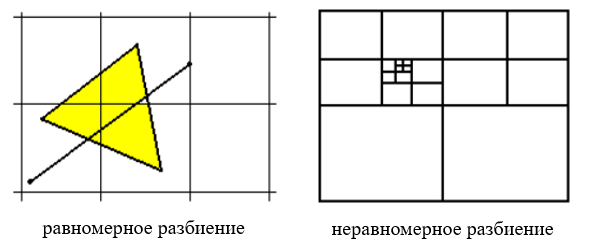
\includegraphics[width=\textwidth]{img/fig_partition.png}
    \caption{Равномерное и неравномерное разбиения пространства объектов}
    \label{fig:partition}
\end{figure}

	\item Иерархические древовидные структуры
	
При работе с большими объемами используются различные древовидные (иерархические) структуры. Стандартными формами таких структур являются восьмеричные (Octrees, для 3D), тетрарные (Quadtrees, для 2D), бинарные или BSP-деревья (Binary Space Partitioning Trees) и деревья ограничивающих тел. Иерархии позволяют упорядочивать грани объектов, производить быстрое и эффективное
отсечение граней, не удовлетворяющих каким-либо из условий.

\begin{enumerate}
	\item Иерархия ограничивающих тел
	
Получается дерево, корнем которого является тело, описанное вокруг всей сцены, а потомками – тела, описанные вокруг первичных, вторичных и др. групп.

Отсечение основного количества объектов происходит уже на ранней
стадии достаточно быстро, ценой всего лишь нескольких проверок.
	\item Иерархии разбиения
	
Каждая клетка исходного разбиения разбивается на части (которые, в свою очередь, так же могут быть разбиты и т.д. При этом каждая клетка разбиения соответствует узлу дерева).

Иерархии (как и разбиения) позволяют достаточно легко и просто
производить частичное упорядочение граней. В результате получается список граней, практически полностью упорядоченный,
что дает возможность применять специальные методы сортировки.
\end{enumerate}

\end{enumerate}

Специальные методы оптимизации:

\begin{enumerate}
	\item Потенциально видимые множества граней (препроцессинг построения PVS)
	\item Метод порталов (PVS "на ходу")
	\item Метод иерархических подсцен (модификация метода порталов)~\cite{tyrlapov}
\end{enumerate}

\subsubsection{Алгоритмы предварительного удаления невидимых линий и поверхностей}



\subsection{Алгоритмы отрисовки теней}

\hspace{1.25cm}


\subsection{Алгоритмы освещения}

\hspace{1.25cm}


\newpage